\chapter{Background}\label{ch:sample-chapter}

\section{Web Proxies}
Web proxy services are tools that allow users to access web content that might be inaccessible because of technical limitations, geographical restrictions or other reasons. They act as intermediaries between the user and the original web content. When a user requests content through a web proxy service, the service retrieves the content from the original source, processes it, and then delivers it to the user. 

A web proxy service is essentially a website that users connect to in order to access other resources on the internet. When someone uses a proxy service, an outside observer can only see that the user is communicating with the proxy service and cannot determine what specific websites or content the user is actually accessing.

For example, Figure \ref{fig:proxy-site} shows the welcome screen of the web proxy service \texttt{proxysite.com}. As shown, the website allows users to enter a URL they want to visit, and they can access that resource while remaining connected to \texttt{proxysite.com}.

\begin{figure}
    \centering
    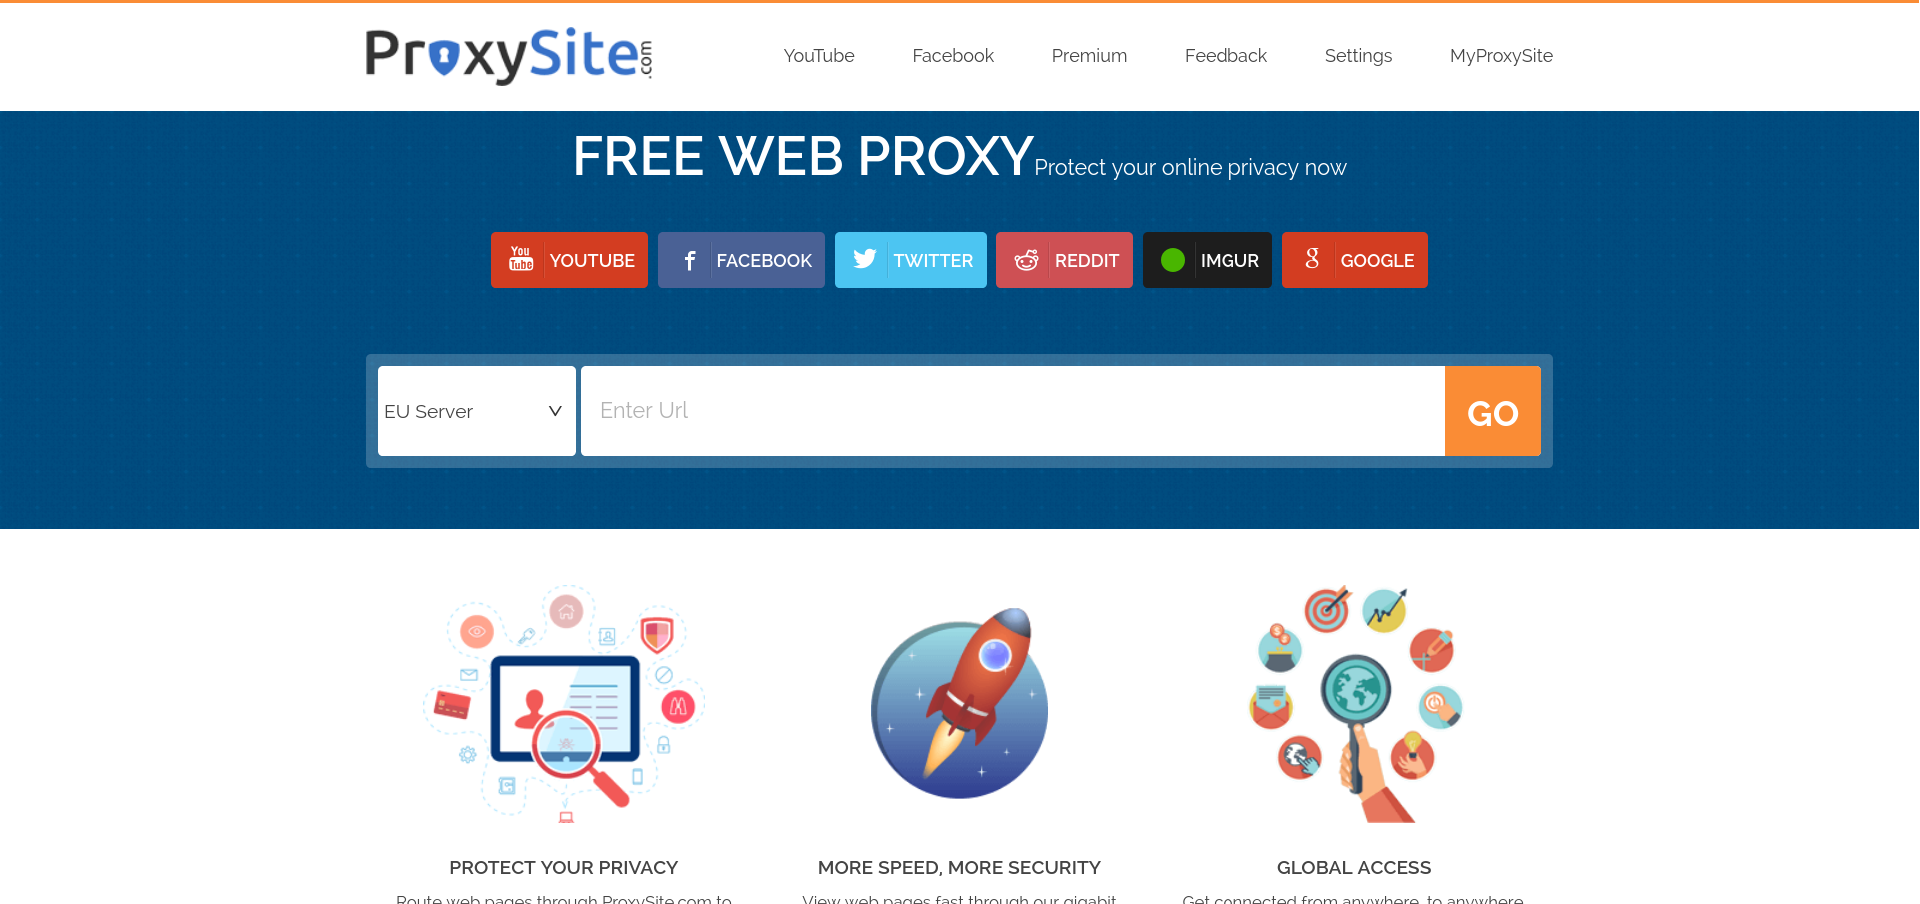
\includegraphics[width=1\linewidth]{media/proxy-site.png}
    \caption{proxysite.com website homepage}
    \label{fig:proxy-site}
\end{figure}

While these services can be very useful, they also come with significant security and privacy risks. Users have to trust the service providers with their potentially sensitive information, as the providers act as a "Man In The Middle" (MITM), meaning they have access to everything the user does online.

\section{Transport Layer Security (TLS)}
Transport Layer Security (TLS)\cite{rfc8446} is a protocol used to ensure secure communication over a computer network. It provides privacy, integrity, and authentication between two communicating applications. TLS is widely used in web browsers, email, messaging, and other applications that require secure data exchange. It uses a combination of symmetric and asymmetric encryption, digital signatures, and certificates to establish a secure connection, authenticate the parties involved, and encrypt the data transmitted. TLS is essential for protecting sensitive information from being intercepted or tampered with during transmission.

\section{Trusted Execution Environments (TEEs)}
A Trusted Execution Environment (TEE) is a security mechanism that allows to isolate code and data from higher-privileged software like the operating system, hypervisor, and BIOS. Any software running outside the TEE is considered untrustworthy. Only code executed within the TEE has the ability to access the data it contains, thereby safeguarding the confidentiality and integrity of this information from untrusted software. Additionally, TEEs often support Remote Attestation (RA), enabling external clients to verify exactly what software is operating inside the TEE.

There are several TEEs that have been developed and adopted in various systems. The following are some of the most common ones:

\begin{itemize}
    \item \textbf{Intel SGX (Software Guard Extensions)}\cite{costan2016intel}: Intel SGX provides isolated memory regions called enclaves, where code and data are protected from access by external processes, including the operating system. Its key feature is fine-grained memory isolation.
    
    \item \textbf{ARM TrustZone}\cite{7809736}: A hardware-based TEE, TrustZone creates two separate execution environments: the secure world and the normal world. It is primarily used in mobile and embedded systems for its simplicity in creating a split environment.
    
    \item \textbf{AMD SEV (Secure Encrypted Virtualization)}\cite{amd-sev}: SEV allows encryption of memory in virtual machines, providing isolation from the hypervisor. Its strength lies in its ability to protect virtualized environments.
    
    \item \textbf{RISC-V Keystone}\cite{lee2019keystone}: An open-source TEE for the RISC-V architecture, Keystone is designed to provide flexibility in TEE configuration. Its modularity and openness make it unique among TEEs.
\end{itemize}

These TEEs provide varying levels of security, tailored for different applications and trust models. Each TEE has distinct features, but all share the common goal of providing an isolated, trusted environment for secure code execution.

\subsection{Intel SGX \& Enclaves}
Intel Software Guard Extensions (SGX) is a set of security-related instruction codes that are built into modern Intel processors. SGX allows developers to create enclaves, which are protected areas of execution in memory. These enclaves are isolated from the rest of the system, including the operating system and hypervisor, providing a high level of security for sensitive code and data. SGX is particularly useful for applications requiring strong protection against both external and internal threats. It enables secure computation, data protection, and integrity assurance, even in potentially compromised environments.

Figure \ref{fig:threath-model-intelSGX} represents the threat model of Intel SGX. The model assumes that all software outside the enclave, including the operating system, hypervisor, and BIOS, may be compromised. Additionally, all the hardware outside the CPU die is considered untrusted.

\begin{figure}[h!]
    \centering
    \begin{tikzpicture}

    % Define colors
    \definecolor{greenblock}{rgb}{0.67, 0.87, 0.55} % Light green
    \definecolor{redblock}{rgb}{1, 0.4, 0.4}        % Light red

    % Ring 3
    \node[rectangle, draw, fill=greenblock, minimum width=2.5cm, minimum height=1cm] (enclave) {\textbf{Enclave}};
    \node[rectangle, draw, fill=redblock, minimum width=2.5cm, minimum height=1cm, right=0.25cm of enclave] (app) {\textbf{App}};

    % Ring 2-0
    \node[rectangle, draw, fill=redblock, minimum width=2.5cm, minimum height=1cm, below=0.25cm of enclave] (vm1) {\textbf{VM OS}};
    \node[rectangle, draw, fill=redblock, minimum width=2.5cm, minimum height=1cm, right=0.25cm of vm1] (vm2) {\textbf{VM OS}};

    % Ring 0
    \node[rectangle, draw, fill=redblock, minimum width=5.25cm, minimum height=1cm, below=1.25cm of vm2.east, anchor=east] (hypervisor) {\textbf{Hypervisor}};

    % Dashed line
    \draw[dashed, below=0.5cm of hypervisor,  minimum width=5.25cm] (-1.2, -3.25) -- (4.05, -3.25);

    % HW
    \node[rectangle, draw, fill=greenblock, minimum width=2.5cm, minimum height=1cm, below=1.5cm of hypervisor.west, anchor=west] (cpu) {\textbf{CPU}};
    \node[rectangle, draw, fill=redblock, minimum width=2.5cm, minimum height=1cm, right=0.25cm of cpu] (dram) {\textbf{DRAM}};
    \node[rectangle, draw, fill=redblock, minimum width=5.25cm, minimum height=1cm, below=1.25cm of cpu.west, anchor=west] (other) {\textbf{Other peripherals}};

    % Title
    \node[anchor=north, above=2.75cm of hypervisor] {\textbf{Intel SGX}};

    % Ring Labels
    \node[anchor=east,  left=0.25cm of enclave] {\textbf{Ring 3}};
    \node[anchor=east, left=0.25cm of vm1] {\textbf{Ring 2-0}};
    \node[anchor=east, left=0.25cm of hypervisor] {\textbf{Ring 0}};
    \node[anchor=east, left=0.25cm of cpu] {\textbf{HW}};
\end{tikzpicture}
    \caption{Intel SGX threat model: green components are trusted, red are untrusted.}
    \label{fig:threath-model-intelSGX}
\end{figure}

\section{Remote Attestation (RA)}
Remote Attestation (RA) is a process that allows one party to verify the integrity and authenticity of software and hardware running on a remote system. It involves generating cryptographic proofs that the code running in a TEE, such as an SGX enclave, is genuine and has not been tampered with. RA ensures that the remote system is in a trusted state before sensitive data or operations are entrusted to it. 

\subsection{Remote Attestation in Intel SGX}
Remote Attestation (RA) in the context of Intel SGX allows an enclave to prove its identity and integrity to a remote party, thereby establishing a secure and trusted communication channel.

\subsubsection{Process Overview}
The RA process involves generating a signed quote by a special enclave known as the Quoting Enclave. This quote is a cryptographic statement that includes information about the enclave's measurement, called \texttt{MRENCLAVE}, which corresponds to the enclave's identity. The measurement is performed by the Intel processor.

\subsubsection{Establishing Secure Communication}
This mechanism ensures that sensitive operations and data exchanges are only conducted with trusted enclaves. Public keys or other data can be securely shared as part of the signed quote. Secure communication between enclaves on the same platform is achieved via local attestation.

\subsubsection{Verification by the Client} \label{sec:verification-client}
The client intending to verify the enclave's identity receives the quote. It first checks whether \texttt{MRENCLAVE} matches the expected value. The client then sends the quote to a remote attestation service, such as the Intel Attestation Service (IAS), for verification. Once the IAS verifies the quote, it provides a signed attestation report that confirms the enclave's authenticity and integrity.

The Intel Attestation Service (IAS) is a cloud-based service provided by Intel that facilitates remote attestation for SGX enclaves. The IAS acts as a trusted third party that verifies the quotes generated by SGX enclaves during the attestation process. It signs the attestation reports with its own Root Certificate Authority (CA).

\subsubsection{Remote Attestation over TLS} 
In \cite{sgx-ra-tls-white-paper}, Remote Attestation (RA) is integrated directly into the TLS protocol. In the proposed design, the enclave itself carries out the verification steps outlined in Section \ref{sec:verification-client}. The key idea is that the enclave retrieves the signed attestation report and provides it to the user, thereby eliminating the need for the user to directly contact the Intel Attestation Service (IAS).

The certificate used by the enclave during the TLS handshake includes, in its extensions section, both the quote and the corresponding signed attestation report. The client can verify this quote using the attestation report. The quote contains not only the identity of the enclave but also the public key corresponding to the private key used to sign the TLS certificate. This final step securely binds the identity of the enclave to the TLS certificate being used.


